
\chapter{Appendix}



\section{Somato-dendritic coupling}\label{sec-somato-dendr}

\cite{urbanczik2014learning} discuss a possible extension to their neuron- and plasticity model, in which the
dendro-somatic coupling transmits voltages in both directions. They show that the plasticity rule requires only minor
adaptations for successful learning under this paradigm. Yet, as described by passive cable theory, the flow between
neuronal compartments is dictated by their respective membrane capacitances. These are calculated from their membrane
areas, which vastly differ in the case of pyramidal neurons. \todo{find a nice citation for this}


15,006 458


will not be considered here. The motivation is, that dendritic membrane area is



\section{Default parameters}
\begin{table}
  \fontsize{12pt}{12pt}\selectfont
  \begin{center}
    \begin{tabular}{p{0.25\textwidth}p{0.6\textwidth}p{0.15\textwidth}}    \hline
      \textbf{Name}                & \textbf{Description}                                                        &
      \textbf{Default}                                                                                                   \\
      \hline

      \\\textbf{Simulation} \\\hline
      \texttt{n\_epochs}           & Number of training iterations                                               &
      $1000$                                                                                                             \\
      \texttt{delta\_t}            & Euler integration step in [ms]                                              & $0.1$
      \\
      \texttt{t\_pres}             & Stimulus presentation time during training [ms]                             & $50$
      \\
      \texttt{out\_lag}            & Lag before recording output during testing [ms]                             & $35$
      \\
      \texttt{dims}                & Network dimensions, i.e. pyramidal neurons per layer                        & [9,
      30, 3]                                                                                                             \\
      \texttt{threads}             & Number of threads for parallel processing                                   & $8$
      \\
      \texttt{test\_interval}      & Test the network every N epochs                                             & $10$
      \\
      \texttt{record\_interval}    & Interval for storing membrane potentials [ms]                               & $1$
      \\
      \texttt{init\_self\_pred}    & Flag to initialize weights to self-predicting state                         &
      \texttt{True}                                                                                                      \\
      \texttt{noise}               & Flag to apply noise to membrane potentials                                  &
      \texttt{False}                                                                                                     \\
      \texttt{sigma}               & Standard deviation for membrane potential noise                             & 0.3
      \\
      \texttt{mode}                & Which dataset to train on. Choice between (bars, mnist, self-pred, teacher) & bars
      \\
      \texttt{store\_errors}       & Flag to compute and store apical and interneuron errors during training     &
      \texttt{False}                                                                                                     \\
      \texttt{network\_type}       & Choice between (numpy, snest, rnest)                                        & snest
      \\
      \texttt{tau\_x}              & Network input filtering time constant [ms]                                  & 0.1   \\
      \texttt{reset}               & Reset method between simulations (0:no reset, 1=soft reset, 2=hard reset)   & 2
      \\

      \\
      \textbf{Neurons}
      \\\hline
      \texttt{latent\_equilibrium} & Flag for whether to use prospective transfer functions                      &
      \texttt{True}                                                                                                      \\
      \texttt{g\_l}                & Somatic leakage conductance [nS]                                            & 0.03
      \\
      \texttt{g\_a}                & Apical compartment coupling conductance [nS]                                & 0.06
      \\
      \texttt{g\_d}                & Basal compartment coupling conductance [nS]                                 & 0.1
      \\
      \texttt{g\_som}              & Output neuron nudging conductance [nS]                                      & 0.06
      \\
      \texttt{g\_l\_eff}           & Effective leakage conductance [nS]                                          &
      \texttt{g\_l+g\_d+g\_a}                                                                                            \\
      \\
      \texttt{g\_lk\_dnd}          & Dendritic leakage [nS]                                                      &
      \texttt{delta\_t}                                                                                                  \\
      \texttt{t\_ref}              & Refractory period [ms]                                                      & 0.0   \\
      \texttt{C\_m\_som}           & Somatic compartment membrane capacitance [pF]                               & 1.0
      \\
      \texttt{C\_m\_bas}           & Basal compartment membrane capacitance [pF]                                 & 1.0
      \\
      \texttt{C\_m\_api}           & Apical compartment membrane capacitance [pF]                                & 1.0
      \\
      \texttt{gamma}               & Linearly scales  activation function $\phi$                                 & 1.0
      \\
      \texttt{beta}                & Exponentially scales  activation function $\phi$                            & 1.0
      \\
      \texttt{theta}               & Shifts  activation function $\phi$                                          & 0.0
      \\

      \\
      \textbf{Synapses}
      \\\hline
      \texttt{wmin\_init}          & Min. initial synaptic weight                                                & -1.0
      \\
      \texttt{wmax\_init}          & Max. initial synaptic weight                                                & 1.0
      \\
      \texttt{Wmin}                & Min. allowed synaptic weight                                                & -4.0
      \\
      \texttt{Wmax}                & Max. allowed synaptic weight                                                & 4.0
      \\
      \texttt{tau\_delta}          & Weight change filter time constant (NEST only) [ms]                         & 1.0
      \\
      
      \texttt{p\_conn}             & Connection probability between populations                                  & 1.0
      \\
      \texttt{eta\_ip}             & Learning rate for $pyr\rightarrow intn$ synapses                            & 0.004
      \\
      \texttt{eta\_pi}             & Learning rate for $intn\rightarrow pyr$ synapses                            & 0.01
      \\
      \texttt{eta\_up}             & Learning rates for feedforwarsd $pyr\rightarrow pyr$ synapses               &
      [0.01, 0.003]                                                                                                      \\
      \texttt{eta\_down}           & Learning rate for feedback $pyr\rightarrow pyr$ synapses                    & 0.0
      \\
    \end{tabular}\caption{Default parameters used in all simulations. }\label{tab-params}
  \end{center}
\end{table}
\section{Integration of the spike-based Urbanczik-Senn plasticity}



Starting with the complete Integral from $t=0$.

\begin{align}
  \dot{W_{ij}}(t)    & = \eta (\phi(u_i) - \phi(\alpha v^{basal}_i(t))) \phi(u_j)                                                     \\
  \Delta W_{ij}(t,T) & = \int_t^T dt' \ \eta \  (\phi(u_i^{t'}) - \phi(\widehat{v_i^{t'}})) \  \phi(u_j^{t'})                         \\
  \Delta W_{ij}(t,T) & = \eta \int_t^T dt' \  (\phi(u_i^{t'}) - \phi(\widehat{v_i^{t'}})) \ \phi(u_j^{t'})                            \\
  V_i^*              & = \phi(u_i^{t'}) - \phi(\widehat{v_i^{t'}})                                                                    \\
  s_j^*              & = \kappa_s * s_j                                                                                               \\
  \Delta W_{ij}(0,t) & =\eta \int_0^t dt' \  \int_0^{t'} dt'' \ \kappa(t'-t'') V_i^\ast (t'') s_j^\ast (t'')                          \\
                     & = \eta \int_0^t dt'' \  \int_{t''}^{t} dt' \ \kappa(t'-t'') V_i^\ast (t'') s_j^\ast (t'')                      \\
                     & = \eta \int_0^t dt'' \  \left[ \tilde{\kappa}(t-t'') - \tilde{\kappa}(0) \right] V_i^\ast (t'') s_j^\ast (t'') \\
\end{align}

With $\tilde{\kappa}$ being the antiderivative of $\kappa$:

\begin{align}
  \kappa(t)         & = \frac{\delta}{\delta t} \tilde{\kappa}(t) \\
  \tilde{\kappa}(t) & = - e^{-\frac{t}{t_{\kappa}}}               \\
\end{align}

The above can be split up into two separate integrals:

Which implies the identities

\begin{align}
  I_1(t_1, t_2 + \Delta t) & = I_1 (t_1, t_2) + I_1 (t_2, t_2 + \Delta t)                                       \\
  I_2(t_1, t_2 + \Delta t) & = e^{- \frac{t_2 - t_1}{\tau_{\kappa}}} I_2 (t_1, t_2) + I_2 (t_2, t_2 + \Delta t)
\end{align}


\begin{align}
  I_2 (t_1, t_2 + \Delta t) & = -\int_{t_1}^{t_2 + \Delta t} dt' \ \tilde{\kappa} (t_2 + \Delta t - t') V_i^\ast (t') s_j^\ast (t')                                        \\
                            & = -\int_{t_1}^{t_2} dt' \ \left[ -e^{- \frac{t_2 + \Delta t - t'}{\tau_\kappa}} \right] V_i^\ast (t') s_j^\ast (t')
  -\int_{t_2}^{t_2 + \Delta t} dt' \ \left[ -e^{- \frac{t_2 + \Delta t - t'}{\tau_\kappa}} \right] V_i^\ast (t') s_j^\ast (t')                                             \\
                            & = -e^{- \frac{ \Delta t}{\tau_\kappa}} \int_{t_1}^{t_2} dt' \ \left[ -e^{- \frac{t_2 - t'}{\tau_\kappa}} \right] V_i^\ast (t') s_j^\ast (t')
  -\int_{t_2}^{t_2 + \Delta t} dt' \ \left[ -e^{- \frac{t_2 + \Delta t - t'}{\tau_\kappa}} \right] V_i^\ast (t') s_j^\ast (t')
\end{align}


Using this we can rewrite the weight change from $t$ to $T$ as:


\begin{align}
  \Delta W_{ij}(t,T) & = \Delta W_{ij}(0,T) - \Delta W_{ij}(0,t)                                               \\
                     & = \eta [-I_2(0,T) + I_1(0,T) + I_2(0,t) - I_1(0,t)]                                     \\
                     & = \eta [I_1(t,T) - I_2(t,T) + I_2(0,t)\left( 1 - e^{- \frac{T-t}{\tau_\kappa}} \right)]
\end{align}

The simplified \cite{sacramento2018dendritic} case would be:

\begin{align}
  \frac{dW_{ij}}{dt} & = \eta (\phi(u_i) - \phi(\hat{v_i})) \phi(u_j)                                         \\
  \Delta W_{ij}(t,T) & = \int_t^T dt' \ \eta \  (\phi(u_i^{t'}) - \phi(\widehat{v_i^{t'}})) \  \phi(u_j^{t'}) \\
  \Delta W_{ij}(t,T) & = \eta \int_t^T dt' \  (\phi(u_i^{t'}) - \phi(\widehat{v_i^{t'}})) \ \phi(u_j^{t'})    \\
  V_i^*              & = \phi(u_i^{t'}) - \phi(\widehat{v_i^{t'}})                                            \\
  s_j^*              & = \kappa_s * s_j
\end{align}


Where $s_i$ is the postsynaptic spiketrain and $V_i^*$ is the error between dendritic prediction and somatic rate and
$h( u )$. The additional nonlinearity $h( u ) = \frac{d}{du} ln \  \phi(u)$ is ommited in our model \todo{should it
  though?}.




Antiderivatives:

\begin{align}
  \int_{-\infty}^x H(t)dt = tH(t) = max(0,t)
\end{align}


\begin{align}
  \tau_l & = \frac{C_m}{g_L} = 10 \\
  \tau_s & = 3
\end{align}

Writing membrane potential to history (happens at every update step of the postsynaptic neuron):



\section{Dendritic leakage conductance}\label{sec-gl-dend}

In order to match the dendritic potential of rate neurons  in the spiking neuron model, a suitable leakage conductance
for dendritic compartments was required. As described in Equation \ref{eq-spiking-basal-compartment}, a dendritic
compartment evolves according to:
\begin{align}
  C_m^{dend} \dot{v}_j^{dend} & = -g_l^{dend} \  v_j^{dend} + \sum_i W_{ji} \    \langle \textit{n}_i \rangle
\end{align}

Under the assumption that the activation of all presynaptic neurons $i$ remains static over time, we can replace the
spontaneous activation $s_i(t)$ with the expected number of spikes per simulation step $\langle \textit{n}_i \rangle =
  r_i \ \Delta t$ (cf. Equation \ref{eq-n-spikes}). Note that these values do not employ matrix notation, but refer to
individual neurons. Next, in order to find the convergence point of the ODE, we set the left side of the equation to $0$
and to solve it:

\begin{align}
  0                        & = -g_l^{dend} \  v_j^{dend} + \sum_i W_{ji} \    r_i \ \Delta t \\
  g_l^{dend} \  v_j^{dend} & = W_{ji} \    r_i \ \Delta t
\end{align}

The instantaneous dendritic potential of rate neurons is given by $v_j^{dend} = \sum_i W_{ji} \ r_i$. Since we are
searching for a parametrization which fulfils this equality in the steady state, the terms drop out from the above
equation. Thus, the correct parametrization for the dendritic leakage conductance remains:
\begin{align}
  g_l^{dend} & = \Delta t
\end{align}

It was shown experimentally that for high values of $\psi$, this parameterization leads to an exact match of dendritic
potentials between the neuron models. It will therefore be assumed as the default throughout all experiments where
spiking neurons are used. \newline

In order to keep the two NEST models as similar as possible, rate neurons evolve according to the same dynamics. Like in
the original implementation, dendrites of rate neurons ought to be fully defined by their inputs at time $t$. This
behaviour is achieved by setting the leakage conductance to $1$ for all dendritic compartments. During network
initialization, dendritic leakage conductances are set to either one of these values depending on the type of neuron
model employed.


\section{Plasticity in feedback connections}\label{sec-feedback-plast}

\todo{move to results}

Within the present model, Pyramidal-to-pyramidal feedback weights evolve according to:

\begin{align}
  \dot{w}_{l}^{down} & = \eta_l^{down} \ ( \phi(u_l^{P}) - \phi(w_l^{down} r_{l+1}^P) )\ \phi(u_{l+1}^{P})^T
\end{align}

The error term in this case differs slightly from the others, but could arguably still be implemented by biological
neurons. An intuitive way to interpret the error term is as the difference between somatic activity and the activity of
a distant apical compartment that is innervated only by superficial pyramidal neurons. Within the NEST implementation,
this distal compartment leaks into the proximal apical compartment ($v^{api}$) with a conductance of $g^{api,dist}=1$.
The separation of pyramidal neuron apical dendrites into a proximal and a distal tree is well documented \citeme. A
difference between plasticity mechanisms for synapses arriving at these two integration zones is plausible, although I
was unable to find prior research supporting this type of plasticity \citeme.  A more sophisticated model of the apical
tree which resembles pyramidal neurons more closely could be a desirable extension to the model.

While the plasticity was successfully implemented in all variants of the model, it did not prove useful for training the
networks during my tests. A strong indicator to the reason behind this is the fact, that the dendritic error for this
rule is nonzero, even in the self-predicting state (cf. Fig. \ref{fig-error-comp-le}). Making these connections
non-plastic led to the best learning performance, and is therefore assumed as the default for all training simulations.
This matches the previous implementations of this network too, which typically set learning rates of these connections
to $0$ with the exception of a few experiments employing steady-state approximations. Note that feedback information is
transmitted through fixed weights in this case. Feedforward weights in turn learn to match these, meaning that the
network effectively implements a type of Feedback alignment \cite{Lillicrap2014}.

\newpage
\section{Supplementary Figures}


\renewcommand{\thefigure}{S\arabic{figure}}
\begin{figure}[h]
  \centering
  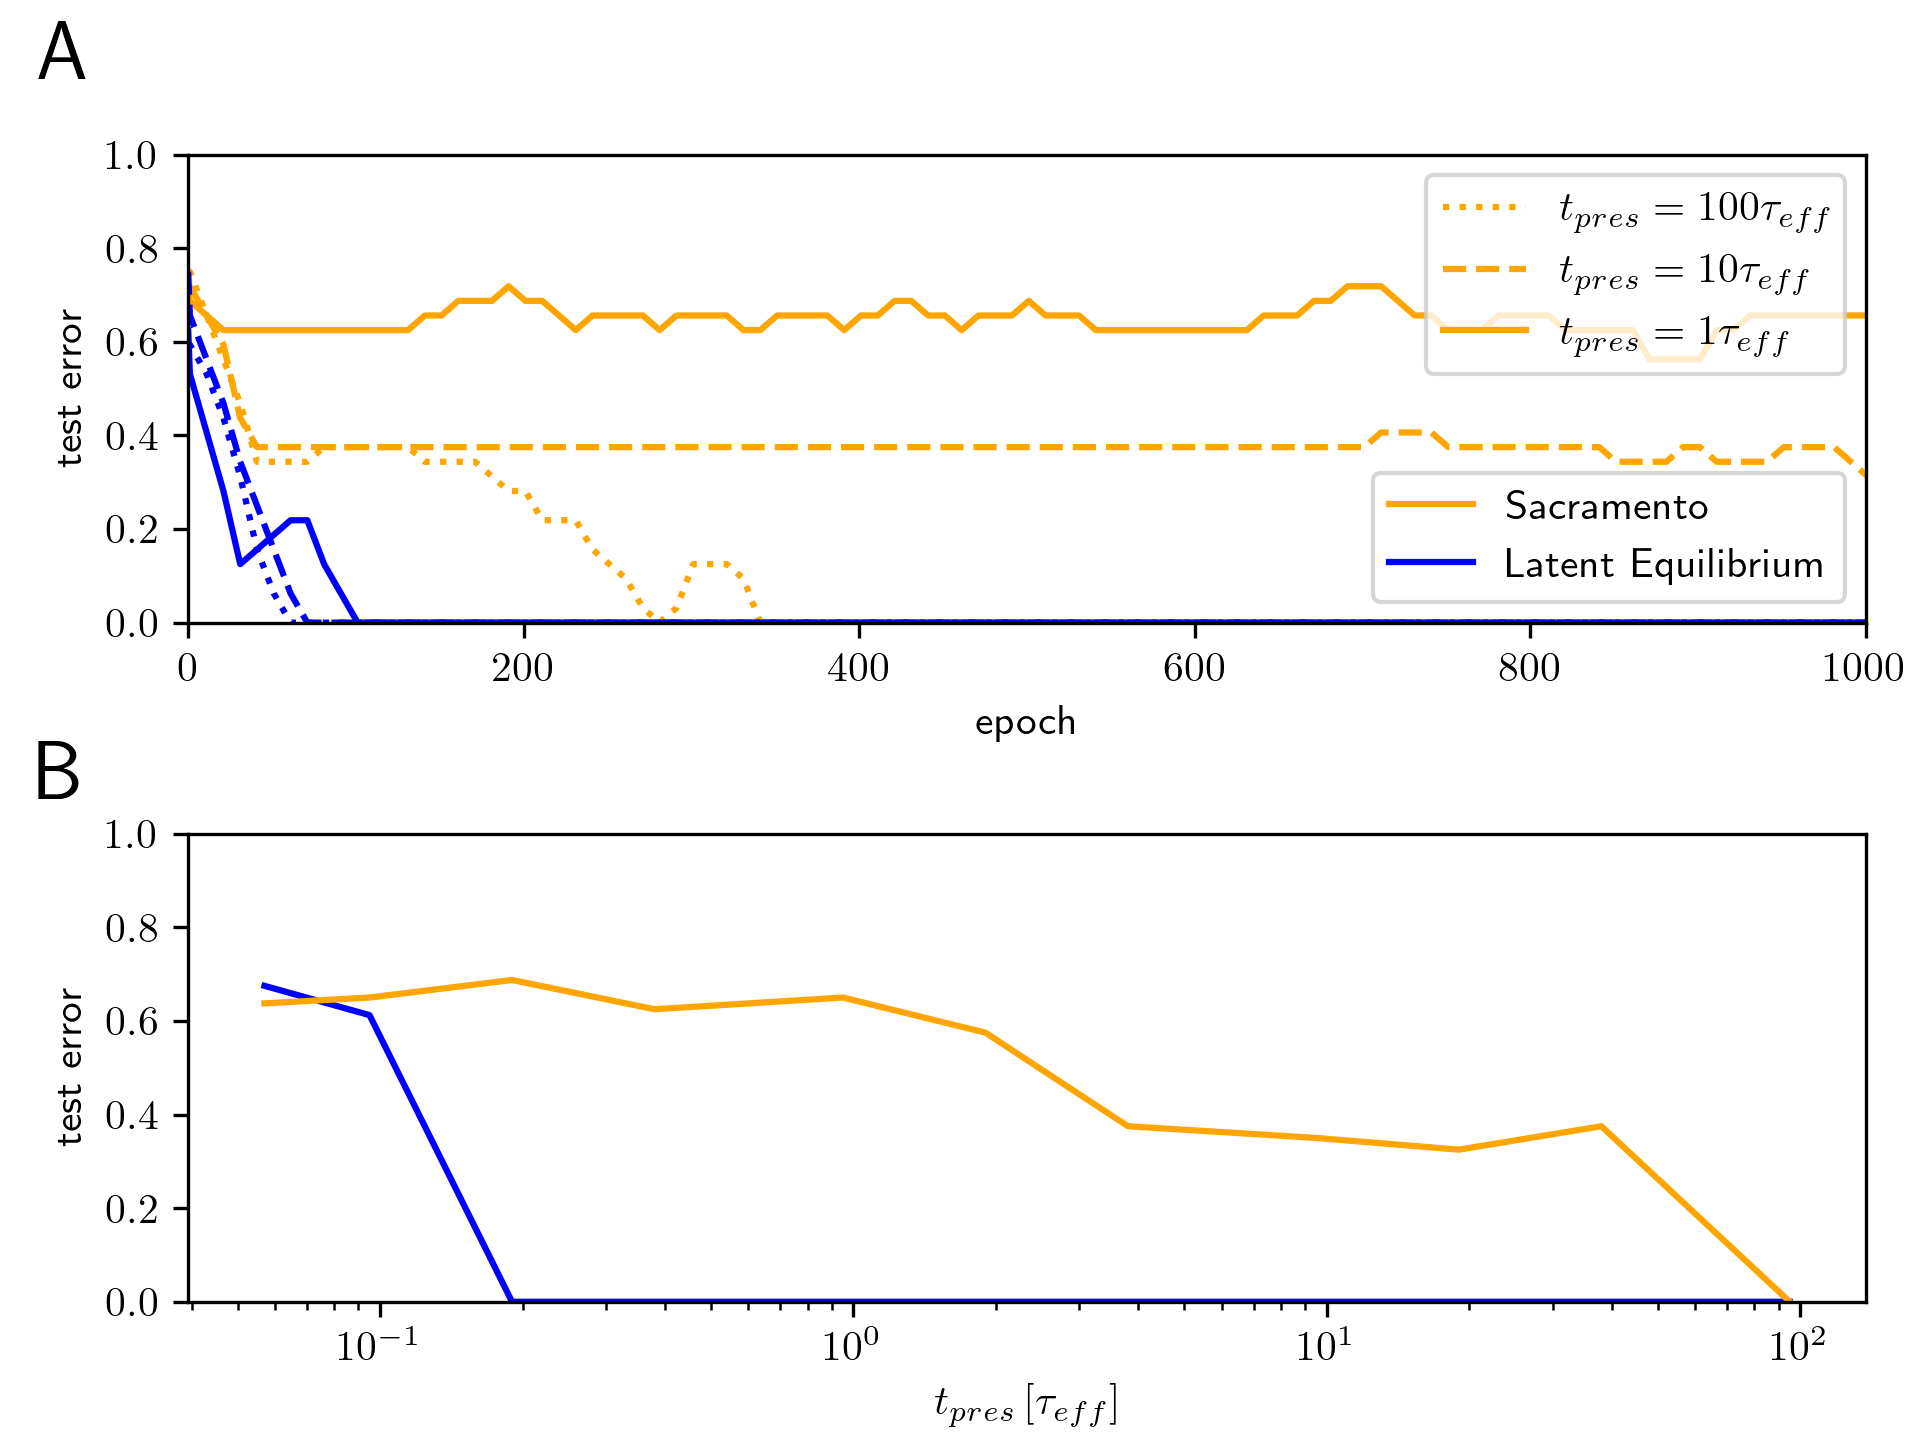
\includegraphics[width=0.9\textwidth]{fig_3_numpy}
  \caption{Replication of Fig. \ref{fig-bars-le-snest} using a slightly modified version of the python code from
    \cite{Haider2021}. Resulting performance matches the original results closely, showing that this version can serve
    as a baseline for comparing performance of the NEST implementation to the original results. Note, how in this
    implementation, presentation time has hardly any effect on the LE network because all updates are instantaneous.
    At the lower end presentation time is only limited by simulation timestep $\Delta t$.}
  \label{fig-bars-le-numpy}
\end{figure}


\begin{figure}[h]
  \centering
  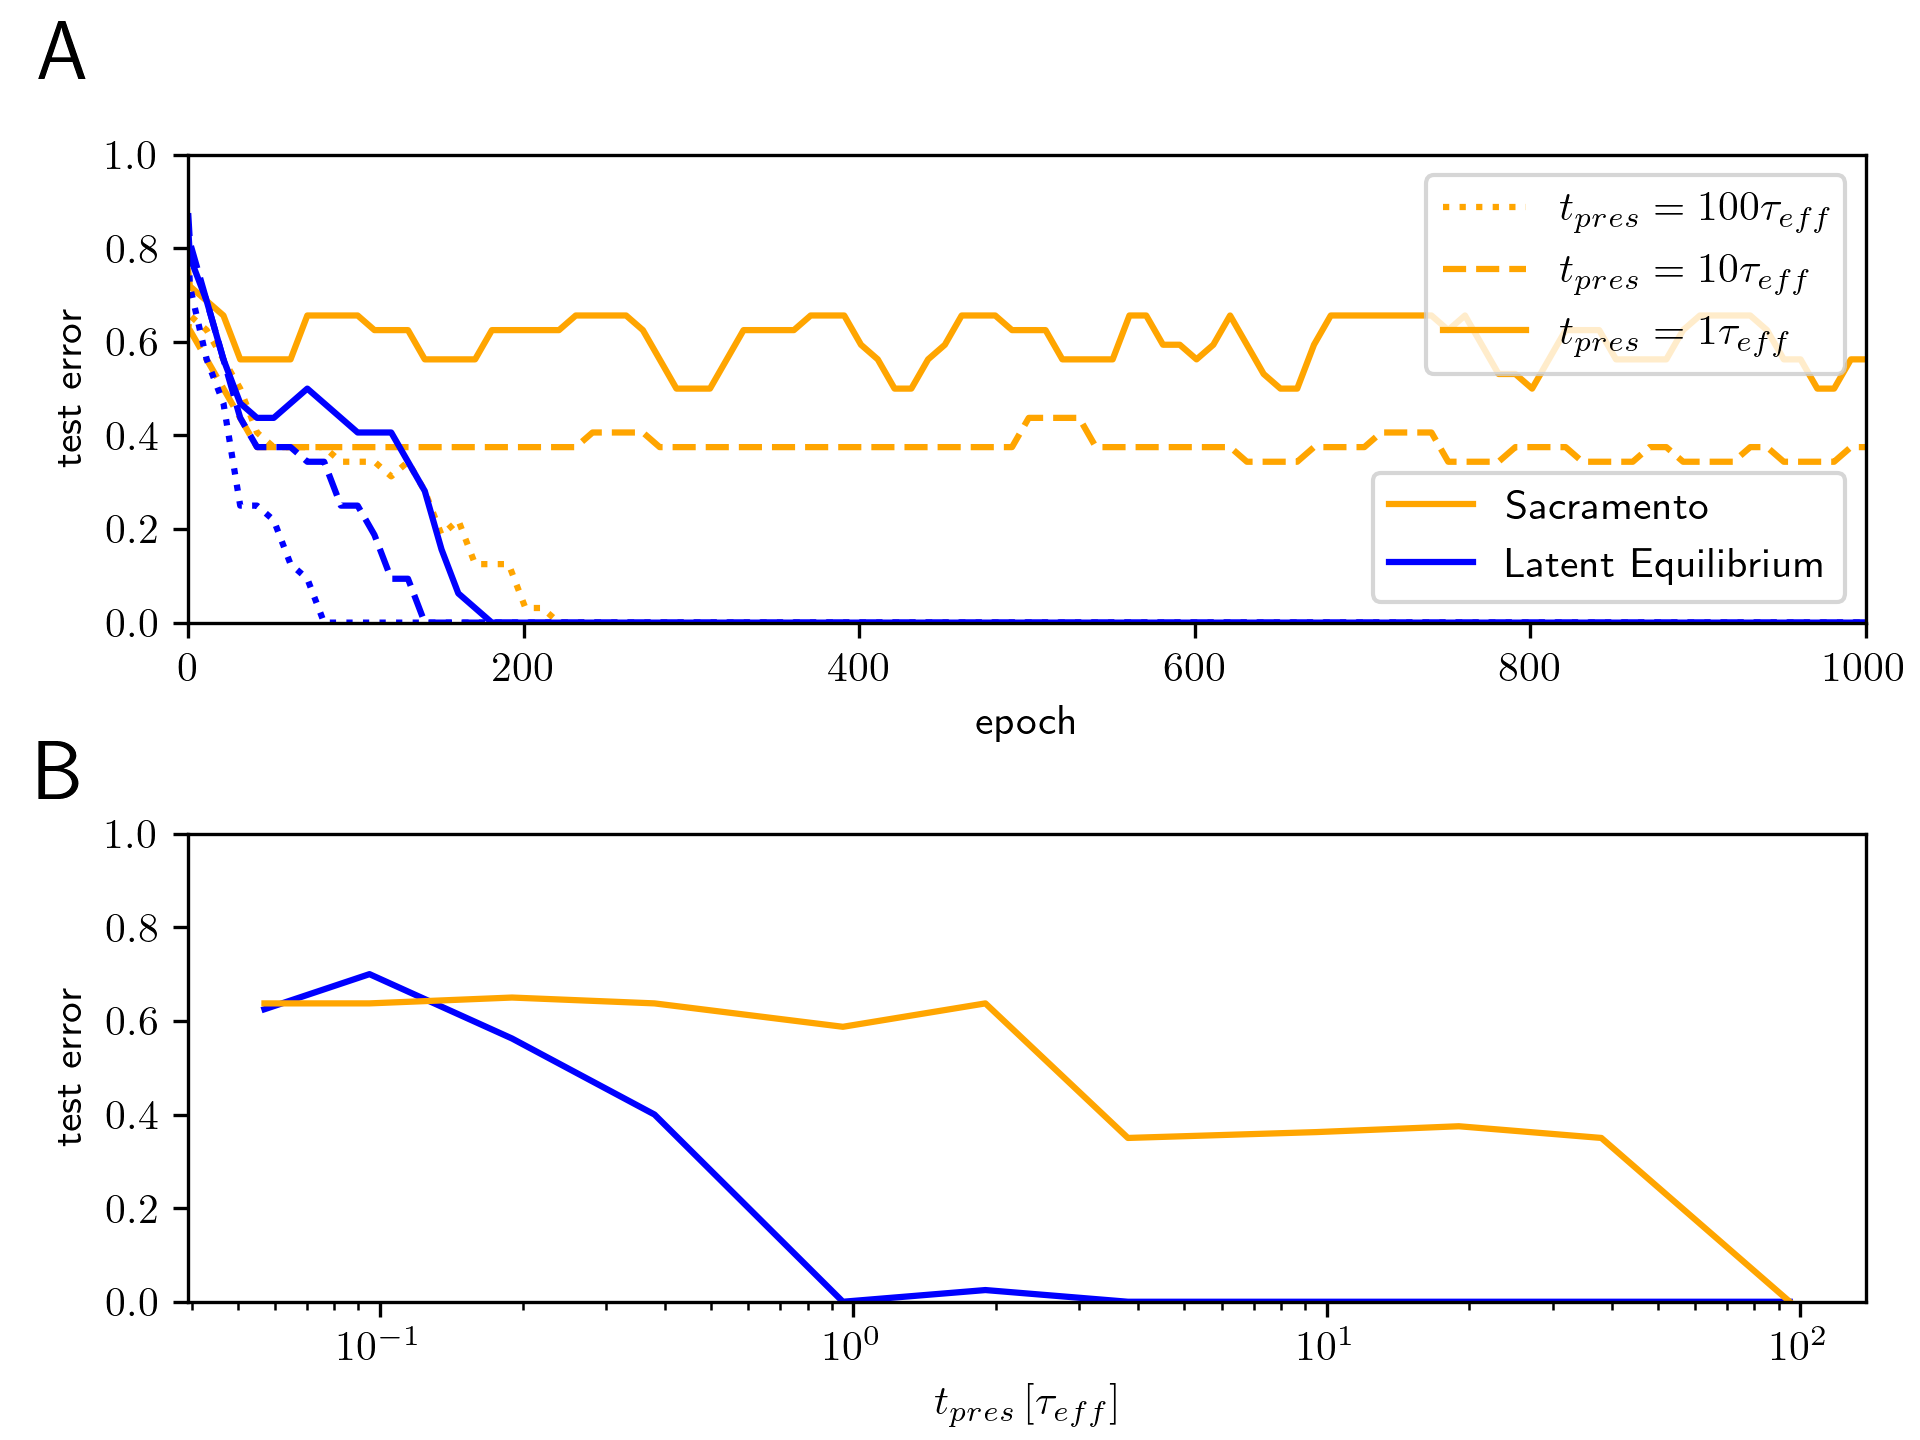
\includegraphics[width=0.9\textwidth]{fig_3_rnest}
  \caption{Replication of Fig. \ref{fig-bars-le-snest} using networks of rate neurons in the NEST simulator. A notable
    difference to the python implementation in Fig. \ref{fig-bars-le-numpy} is, that this version does not handle very
    low presentation times as well. This can likely be traced back to the synaptic delay enforced by NEST, which imposes
    an upper bound on network relaxation time. Besides that, performance of the two variants is very similar.}
  \label{fig-bars-le-rnest}
\end{figure}


